%% chapter12_slides.tex
%% Beamer slides for Chapter 12: Using e-values to combine dependent p-values
%% "Hypothesis Testing with E-Values" by Aaditya Ramdas and Ruodu Wang (arXiv:2410.23614)
%% Reader-friendly style: intuition first, step-by-step derivations, worked numeric example
%% Compiled with: pdflatex -interaction=nonstopmode chapter12_slides.tex  (twice)
\documentclass[aspectratio=169,10pt]{beamer}

\usetheme{Madrid}
\usecolortheme{seahorse}
\usefonttheme{professionalfonts}

%% ── Packages ──────────────────────────────────────────────────────────────
\usepackage{amsmath,amssymb,amsfonts}
\usepackage{mathtools}
\usepackage{graphicx}
\usepackage{booktabs}
\usepackage{xcolor}
\usepackage{listings}

\graphicspath{{figures/}}

%% ── Python listing style ─────────────────────────────────────────────────
\lstdefinestyle{pycode}{
  language=Python,
  basicstyle=\ttfamily\scriptsize,
  numbers=left,
  numberstyle=\tiny\color{gray},
  frame=single,
  backgroundcolor=\color{gray!7},
  keywordstyle=\color{blue!70!black}\bfseries,
  commentstyle=\color{green!50!black}\itshape,
  stringstyle=\color{orange!80!black},
  showstringspaces=false,
  breaklines=true,
  tabsize=2,
  xleftmargin=1.5em,
  framexleftmargin=1.5em,
  aboveskip=4pt,
  belowskip=4pt,
}
\lstset{style=pycode}

%% ── Metadata ─────────────────────────────────────────────────────────────
\title[E-Values -- Ch.12]{Hypothesis Testing with E-Values}
\subtitle{Chapter 12: Using E-Values to Combine Dependent P-Values}
\author{Based on Ramdas \& Wang}
\date{}

\setbeamertemplate{footline}[frame number]
\setbeamertemplate{navigation symbols}{}

%% ── Macros ────────────────────────────────────────────────────────────────
\newcommand{\PP}{\mathbb{P}}
\newcommand{\EE}{\mathbb{E}}
\newcommand{\RR}{\mathbb{R}}
\newcommand{\calP}{\mathcal{P}}
\newcommand{\calF}{\mathcal{F}}
\newcommand{\calK}{\mathcal{K}}
\newcommand{\calU}{\mathfrak{U}}
\newcommand{\indic}[1]{\mathbf{1}_{\{#1\}}}
\newcommand{\bp}{\mathbf{p}}

\begin{document}

%% =========================================================================
\begin{frame}
  \titlepage
\end{frame}

%% =========================================================================
\begin{frame}{Where we are}
  \begin{itemize}
    \item \textbf{Chapters 8--11} developed \emph{e-merging}: combining several e-values $E_1,\dots,E_K$ into one e-value. The punchline there: this is \emph{easy} under arbitrary dependence -- e.g.\ the plain average $\tfrac1K\sum_k E_k$ is already valid, by linearity of expectation alone, no matter how the $E_k$ depend on each other.
    \item \textbf{Chapter 12} asks the analogous question for \emph{p-values}: given $P_1,\dots,P_K$ that are p-values for the same or related nulls, possibly with completely unknown/adversarial dependence, how do we combine them into a single valid p-value?
    \item Surprise: this is \emph{much harder} for p-values than for e-values -- and the clean way to solve it is to \emph{convert p-values to e-values, merge those, and convert back}.
    \item Roadmap:
    \begin{itemize}
      \item 12.1: the arithmetic mean of p-values, and why you must multiply it by 2;
      \item 12.2: general merging functions for p-values under arbitrary dependence, and why \emph{all} of them secretly come from e-values;
      \item 12.3: what changes if the p-values are \emph{exchangeable};
      \item 12.4: what changes if you are willing to \emph{randomize}.
    \end{itemize}
  \end{itemize}
\end{frame}

%% =========================================================================
\begin{frame}[allowframebreaks]{Notation you'll need}
  \begin{block}{Setup (recap from Ch.\ 8, 11)}
    Fix an atomless null probability measure $\PP$ (results extend to a general null class $\calP$) and an integer $K\ge2$. We consider $K$ \emph{p-variables} $P_1,\dots,P_K$ for $\PP$, i.e.\ each satisfies $\PP(P_k\le t)\le t$ for all $t\in[0,1]$, and $K$ \emph{e-variables} $E_1,\dots,E_K$, i.e.\ each satisfies $\EE^\PP[E_k]\le1$. Write $\bp=(p_1,\dots,p_K)$, $\calK=\{1,\dots,K\}$, and let $\calU$ be the set of all p-variables for $\PP$.
  \end{block}

  \begin{block}{``Arbitrary dependence'' -- what this phrase actually means}
    Nothing at all is assumed about the \emph{joint} law of $(P_1,\dots,P_K)$ (equivalently, of $(E_1,\dots,E_K)$) beyond each coordinate being marginally valid on its own. We must build procedures that work under the \emph{worst-case} dependence structure (copula) -- including cases where the $P_k$ are deterministic functions of one another. This is exactly the same ``arbitrary dependence'' regime used for e-merging in Chapters 8 and 11; the difference is that p-values behave much worse than e-values under it.
  \end{block}

  \begin{block}{P-merging function (Definition 12.9)}
    A \emph{p-merging function} of $K$ p-values is an increasing Borel map $F:[0,\infty)^K\to[0,\infty)$ such that $F(P_1,\dots,P_K)$ is itself a p-variable \emph{for every choice} of p-variables $P_1,\dots,P_K$ -- i.e.\ valid under arbitrary dependence among them. $F$ is \emph{symmetric} if permuting the inputs doesn't change the output, \emph{homogeneous} if $F(\lambda\bp)=\lambda F(\bp)$ for $\lambda\in(0,1]$ (with $F(\bp)\le1$), and \emph{admissible} if no other p-merging function is uniformly at least as small (i.e.\ it cannot be improved).

    \emph{Plain English:} a p-merging function is a formula that eats $K$ p-values and outputs a single number that is guaranteed to be a valid p-value, \textbf{no matter how} the $K$ inputs are statistically entangled.
  \end{block}

  \framebreak

  \begin{block}{Calibrators (recap from Ch.\ 2)}
    A \emph{calibrator} is a decreasing function $f:[0,\infty)\to[0,\infty]$ with $\int_0^1 f(p)\,\mathrm{d}p\le1$ and $f\equiv0$ on $(1,\infty)$. For any p-variable $P$, $f(P)$ is an e-variable: $\EE^\PP[f(P)]\le\int_0^1 f(p)\,\mathrm{d}p\le1$. Calibrators are exactly the ``p-value $\to$ e-value'' converters we will lean on throughout this chapter. $f$ is \emph{convex} if it is a convex function on $[0,1]$ -- this extra structure is what makes \emph{averaging} p-values (rather than just e-values) work out, as we will see in 12.1.
  \end{block}

  \begin{block}{Exchangeability -- explained plainly}
    $(P_1,\dots,P_K)$ is \emph{exchangeable} if, for every permutation $\pi$ of $\{1,\dots,K\}$, $(P_{\pi(1)},\dots,P_{\pi(K)})$ has the \emph{same joint distribution} as $(P_1,\dots,P_K)$.

    \emph{Analogy:} imagine drawing $K$ cards from a shuffled deck and writing down their values \emph{in the order you drew them}. The values can be highly dependent (e.g.\ correlated because they came from the same deck) -- but relabeling/permuting the order in which you recorded them does not change anything statistically, because the deck was shuffled. Exchangeability is a much weaker, more common assumption than independence: e.g.\ p-values from repeated random sample-splits of the \emph{same} dataset are exchangeable (the split itself is symmetric/random) but typically far from independent.
  \end{block}

  \begin{block}{Randomized test (recap)}
    A test may use extra external randomness: an auxiliary random variable $U$ (or $V$), independent of the data, typically $\mathrm{Unif}[0,1]$ or a p-variable in its own right. A randomized level-$\alpha$ test rejects according to a rule $\phi(\text{data},U)\in\{0,1\}$ with $\EE^\PP[\phi]\le\alpha$. Randomization lets us build \emph{sharper} (smaller, more powerful) merged p-values than any deterministic rule can achieve, at the cost of an extra coin flip that two people analyzing the same data might not agree on.
  \end{block}
\end{frame}

%% =========================================================================
\begin{frame}{Section 12.1 -- Intuition: why does the factor $2$ appear?}
  \begin{itemize}
    \item The most natural way to combine $K$ p-values is to average them: $\bar P = \tfrac1K\sum_k P_k$. Intuitively small $\bar P$ = lots of combined evidence against $H_0$.
    \item But $\bar P$ itself is \emph{not} a valid p-value in general! Even for $K$ i.i.d.\ $\mathrm{Unif}[0,1]$ p-values, the law of large numbers concentrates $\bar P$ tightly around $1/2$ -- so $\PP(\bar P\le0.4)$ can be tiny, but $\PP(\bar P\le0.5)\approx1$, wildly violating $\PP(\bar P\le t)\le t$ for $t$ near $1/2$.
    \item The fix, remarkably, needs only a factor of exactly $2$: \emph{twice} the average of any p-values is always a valid p-value, however they depend on each other.
    \item \textbf{Why $2$ and not, say, $1.5$ or $3$?} This is exactly the same ``$1/\alpha$'' scaling that appears in \textbf{Markov's inequality} for e-values: a p-to-e calibrator must integrate to $1$ over $[0,1]$, and the specific ``triangular'' calibrator $f(p)=(2-2p)_+$ is the (up to the extremal boundary) canonical choice with $\int_0^1 f=1$ that is also \emph{linear}, hence compatible with averaging. Chasing this calibrator through Markov's inequality is precisely how the factor $2$ is born -- we derive this in full on the next slides.
  \end{itemize}
\end{frame}

%% =========================================================================
\begin{frame}[allowframebreaks]{12.1 The arithmetic mean of p-values}
  \begin{block}{Proposition 12.1 \& Definition 12.2: average p-variables}
    A random variable $P$ is an \emph{average p-variable} for $\PP$ if $\EE^\PP[(v-P)_+]\le v^2/2$ for all $v\in(0,1)$. Equivalently (Proposition 12.1), $P$ is the arithmetic mean of finitely many p-variables, or a (possibly continuous) mixture of p-variables, or satisfies $\EE^\PP[g(P)]\ge\int_0^1g(u)\,\mathrm{d}u$ for every increasing concave $g$.

    \emph{Plain English:} an average p-variable is anything that arises as an average (in a suitably general sense) of genuine p-values. Every p-variable is also an average p-variable (take $K=1$), but not conversely.
  \end{block}

  \begin{block}{Proposition 12.4: the factor 2, and why it can't be improved}
    An average p-variable is \emph{not necessarily} a p-variable, but \emph{twice} an average p-variable \emph{always is}. Moreover the factor $2$ is sharp: for any $\gamma<2$, $\gamma P$ fails to be a p-variable for some average p-variable $P$.

    \emph{Extremal example:} let $U\sim\mathrm{Unif}[0,1]$. Both $U$ and $1-U$ are p-variables, so their average, the \emph{constant} $1/2$, is an average p-variable -- and no constant smaller than $1$ (i.e.\ no $\gamma/2$ with $\gamma<2$) can be a valid p-variable, since a constant $c<1$ has $\PP(c\le t)=0$ for $t<c$ but $=1\ge t$ once $t\ge c$, which already forces $c\ge1$ for genuine validity at all $t$... concretely this construction is why the constant multiplier cannot be pushed below $2$.
  \end{block}

  \framebreak

  \begin{block}{Theorem 12.6: the calibration bridge between p-values, e-values, and average p-values}
    For an average p-variable $P$, $f(P)$ is an e-variable for \emph{any} calibrator $f$ that is \emph{convex} on $[0,1]$. Conversely, for any e-variable $E$, $(2E)^{-1}\wedge1$ is an average p-variable.
  \end{block}

  \begin{block}{The three-way calibration relationships}
    \begin{itemize}
      \item p-value $\to$ e-value: $e=f(p)$ for any calibrator $f$ (Ch.\ 2).
      \item e-value $\to$ p-value: $p = e^{-1}\wedge1$ (the unique admissible choice, Ch.\ 2).
      \item average p-value $\to$ e-value: $e=f(p^*)$, needs $f$ \emph{convex} (Thm.\ 12.6).
      \item e-value $\to$ average p-value: $p^*=(2e)^{-1}\wedge1$ (Thm.\ 12.6).
      \item p-value $\to$ average p-value: trivial, $p^*=p$ (a p-value is already one).
      \item average p-value $\to$ p-value: $p=(2p^*)\wedge1$ (Prop.\ 12.4).
    \end{itemize}
    Composing the last two rows (average p-value $\to$ e-value $\to$ average p-value $\to$ p-value) recovers exactly the ordinary e-to-p calibration $e\mapsto e^{-1}\wedge1$ -- \textbf{average p-values sit exactly halfway between p-values and e-values.}
  \end{block}

  \framebreak

  \begin{block}{Theorem 12.8: turning average p-values into level-$\alpha$ tests}
    Let $V\ge0$ be independent of $P$ with $\EE^\PP[V\wedge1]\le\alpha$. (i) If $P$ is a genuine p-variable, $\indic{P\le V}$ is a level-$\alpha$ test. (ii) If $P$ is only an \emph{average} p-variable and $V$ has a decreasing density, $\indic{P\le V}$ is \emph{still} a level-$\alpha$ test. In particular, for $U\sim\mathrm{Unif}[0,1]$ independent of $P$, $\indic{P\le2\alpha U}$ is a level-$\alpha$ test for $\calP$.

    \emph{Deterministic fallback:} without randomization, $\indic{(P_1+\cdots+P_K)/K\le2\alpha}$ is a (weaker but simpler) level-$\alpha$ test -- this is exactly ``twice the average, compared to $\alpha$.''
  \end{block}

  \begin{block}{Mid p-values and posterior predictive p-values (12.1.2), briefly}
    Two important special cases of average p-variables: \emph{mid p-values} $P_T=\tfrac12F(T-)+\tfrac12F(T)$ for a discrete test statistic $T$ (the standard fix for conservative discrete tests), and \emph{posterior predictive p-values} $P_B=\PP(D(X',\psi)\ge D(X,\psi)\mid X)$ in Bayesian analysis, obtained by averaging ordinary p-variables over a posterior distribution of an unknown parameter (Proposition 12.1(ii)). Both are average p-variables but generally \emph{not} p-variables themselves -- exactly the phenomenon this section is built around.
  \end{block}
\end{frame}

%% =========================================================================
\begin{frame}{Step-by-step: how e-values recover ``twice the average'' (KEY INSIGHT)}
  \begin{block}{Goal}
    Show, from scratch, that $2\bar P:=\tfrac{2}{K}\sum_{k=1}^K P_k$ is a valid p-value for \emph{arbitrarily dependent} p-variables $P_1,\dots,P_K$ -- using only calibration to e-values + Markov's inequality (no direct probabilistic argument about $\bar P$'s distribution needed!).
  \end{block}
  \begin{block}{Step 1 -- calibrate each $P_k$ to an e-value, at a trial level $\alpha$}
    Fix a candidate level $\alpha\in(0,1)$. The map $p\mapsto(2-2p)_+$ is a convex calibrator ($\int_0^1(2-2p)\mathrm{d}p=1$, and it vanishes for $p\ge1$). By the calibrator-rescaling property (Ch.\ 2, Prop.\ 2.6), so is $p\mapsto\gamma(2-2\gamma p)_+$ for any $\gamma\ge1$; hence
    \[
      E_k \;:=\; \frac{(2-2P_k/\alpha)_+}{\alpha} \qquad \text{is a genuine e-variable: } \EE^\PP[E_k]\le1, \text{ for each } k.
    \]
  \end{block}
  \begin{block}{Step 2 -- average the e-values (valid under ANY dependence!)}
    By linearity of expectation \emph{alone} -- no assumption on how $E_1,\dots,E_K$ depend on each other -- $\bar E:=\tfrac1K\sum_kE_k$ satisfies $\EE^\PP[\bar E]\le1$ too. This is the chapter-8 lesson: \emph{averaging e-values is always safe under arbitrary dependence.}
  \end{block}
\end{frame}

%% =========================================================================
\begin{frame}{Step-by-step, continued}
  \begin{block}{Step 3 -- apply Markov's inequality}
    Since $\bar E\ge0$ and $\EE^\PP[\bar E]\le1$, Markov's inequality gives, for every $\alpha\in(0,1)$,
    \[
      \PP\!\left(\bar E \ge \frac1\alpha\right) \;\le\; \alpha\cdot\EE^\PP[\bar E] \;\le\; \alpha.
    \]
  \end{block}
  \begin{block}{Step 4 -- unwind the algebra}
    \[
      \bar E\ge\frac1\alpha \iff \frac1K\sum_k\frac{(2-2P_k/\alpha)_+}{\alpha}\ge\frac1\alpha \iff \frac1K\sum_k(2-2P_k/\alpha)_+ \ge 1.
    \]
    If every $P_k\le\alpha$ (no clipping by $(\cdot)_+$), this simplifies:
    \[
      \frac1K\sum_k\Big(2-\frac{2P_k}\alpha\Big)\ge1 \iff 2-\frac2\alpha\cdot\frac1K\sum_kP_k\ge1 \iff \frac2K\sum_kP_k \le \alpha \iff 2\bar P\le\alpha.
    \]
  \end{block}
  \begin{block}{Step 5 -- conclusion}
    Combining Steps 3--4: $\PP(2\bar P\le\alpha) \le \PP(\bar E\ge1/\alpha) \le \alpha$ for every $\alpha\in(0,1)$ (the first inequality can be strict due to clipping, but the bound survives regardless). \textbf{This is exactly Proposition 12.4} -- recovered purely via calibration + Markov, with no dependence assumption anywhere. The ``2'' is precisely the constant baked into the calibrator $f(p)=(2-2p)_+$, which in turn is forced by $\int_0^1f=1$ and $f$ vanishing exactly at $p=1$.
  \end{block}
\end{frame}

%% =========================================================================
\begin{frame}{Running example, part 1: $K=4$ dependent p-values, the direct route}
  \begin{block}{Setup}
    Four (arbitrarily dependent -- e.g.\ from overlapping/correlated sub-studies) p-values:
    \[
      p_1=0.02,\quad p_2=0.15,\quad p_3=0.30,\quad p_4=0.60.
    \]
  \end{block}
  \begin{block}{Classical route: just average and double}
    \[
      \bar p = \frac{0.02+0.15+0.30+0.60}{4} = \frac{1.07}{4} = 0.2675, \qquad 2\bar p = 0.535.
    \]
    By Proposition 12.4, \textbf{$0.535$ is a valid merged p-value}, regardless of how $P_1,\dots,P_4$ depend on each other -- e.g.\ even if they arose from four highly overlapping analyses of the same data.
  \end{block}
  \begin{block}{Sanity check against a naive competitor}
    Bonferroni ($K\min(p_k)=4\times0.02=0.08$) is also valid but far more conservative here since one very small p-value gets diluted by three large ones; the averaging rule rewards \emph{several moderately small} p-values, Bonferroni rewards a \emph{single very small} one.
  \end{block}
\end{frame}

%% =========================================================================
\begin{frame}{Running example, part 1 continued: the e-value route lands in the same place}
  \begin{block}{Step 1: calibrate each $p_k$ to an e-value at trial level $\alpha=0.535$}
    Using $E_k=(2-2p_k/\alpha)_+/\alpha$ with $\alpha=0.535$:
    \[
      \begin{array}{llll}
        E_1 = 3.599, & E_2 = 2.690, & E_3 = 1.642, & E_4 = 0 \ \ (\text{since } p_4/\alpha=1.1215>1,\text{ clipped}).
      \end{array}
    \]
  \end{block}
  \begin{block}{Step 2: average, then compare to $1/\alpha$}
    \[
      \bar E = \frac{3.599+2.690+1.642+0}{4} = 1.983, \qquad \frac1\alpha=\frac1{0.535}=1.869.
    \]
    Indeed $\bar E=1.983\ge1.869=1/\alpha$: the event that certifies validity of $\alpha=0.535$ (Step 4--5 of the derivation) actually holds for these numbers -- \textbf{the e-value route and the direct route certify the very same merged p-value}, $0.535$.
  \end{block}
  \begin{block}{Bonus: a sharper (admissible) calibrator does slightly better}
    Solving the general merging formula (Section 12.2, Example 12.21) with the \emph{same} calibrator $f(p)=(2-2p)_+$ used directly (not just as a validity check) gives the tighter merged p-value $F(\bp)=0.47 < 0.535$ -- see the Python cell below.
  \end{block}
\end{frame}

%% =========================================================================
\begin{frame}[fragile]{Python: 12.1 -- validating $2\bar P$ under strong dependence}
  \begin{lstlisting}
import numpy as np
from scipy.stats import norm
rng = np.random.default_rng(2024)

# Running example numbers
p = np.array([0.02, 0.15, 0.30, 0.60])
alpha = 2 * p.mean()
print(f"2*mean = {alpha:.3f}")                      # 0.535

def f_calibrator(x):
    return np.clip(2.0 - 2.0*x, 0.0, None)           # convex calibrator (2-2p)_+

E = f_calibrator(p/alpha) / alpha                    # e-values at trial level alpha
print("e-values:", np.round(E, 3), " mean(E) =", round(E.mean(), 3),
      " 1/alpha =", round(1/alpha, 3))                # mean(E) >= 1/alpha  -> confirms validity

# --- Strong-dependence simulation (K=8, anti-dependent halves) ---
K, N, rho = 8, 50000, 0.95
W = rng.standard_normal(N)
eps = rng.standard_normal((N, K))
loadings = np.where(np.arange(K) < K//2, rho, -rho)  # half +rho, half -rho
Z = loadings * W[:, None] + np.sqrt(1-rho**2) * eps
P = norm.cdf(Z)                                       # each column marginally Unif(0,1)
twice_mean = np.minimum(2*P.mean(axis=1), 1.0)

for a in [0.05, 0.1, 0.2, 0.5]:
    print(f"alpha={a:.2f}: empirical P(2*mean<=alpha) = {(twice_mean<=a).mean():.4f}  (must be <= {a})")
  \end{lstlisting}
\end{frame}

%% =========================================================================
\begin{frame}{Figure: $2\bar P$ stays valid even under strong (constructed) dependence}
  \centering
  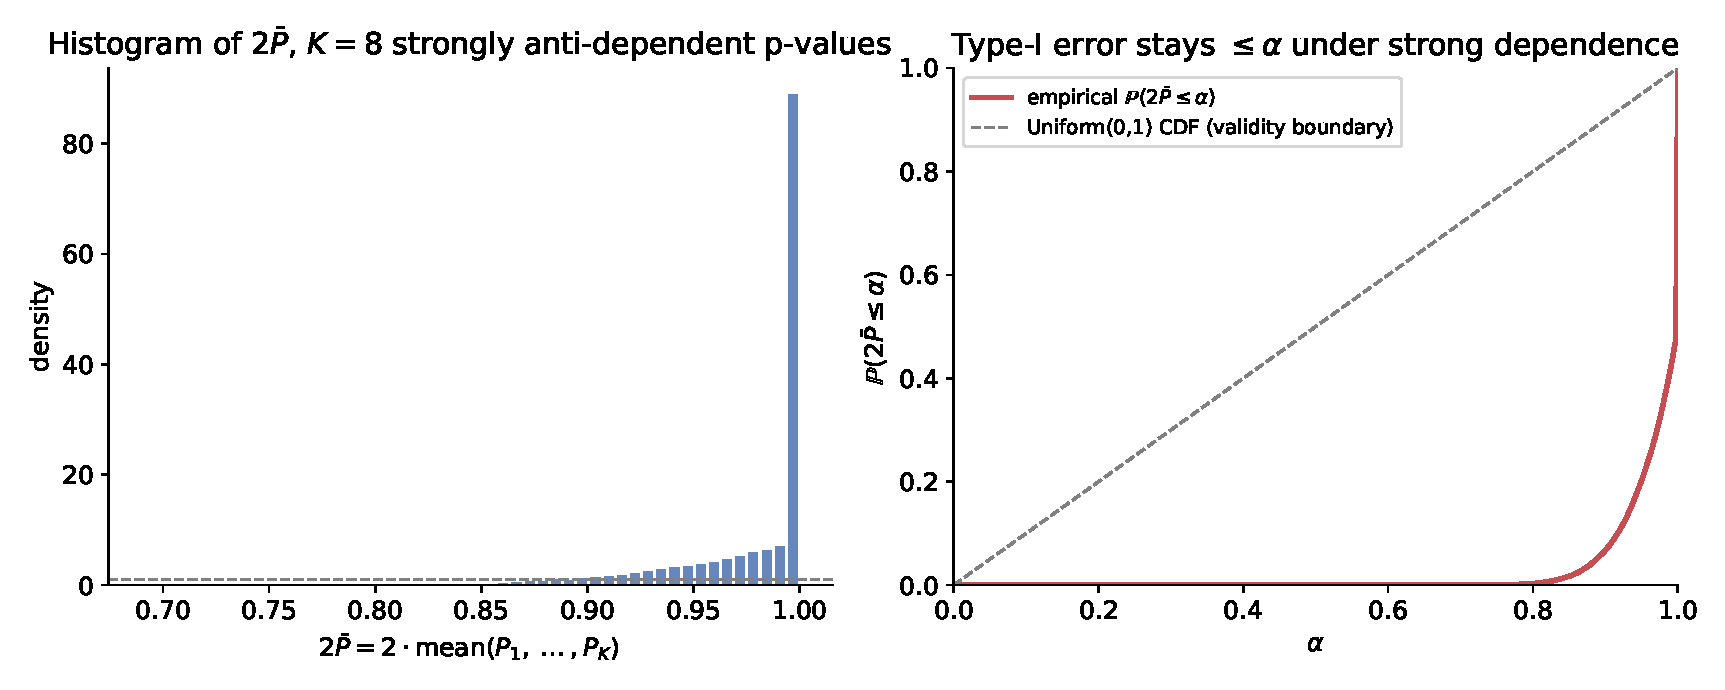
\includegraphics[width=0.95\linewidth]{fig_meanpvalue_validity.pdf}\\
  \small Left: histogram of $2\bar P$ for $K=8$ p-values built to be strongly \emph{anti}-dependent across two halves (a Gaussian-copula construction, loadings $\pm0.95$ on a common factor) -- the same qualitative mechanism as the extremal example $P_1=U,\,P_2=1-U$ behind Proposition 12.4. Right: the empirical CDF of $2\bar P$ never crosses above the Uniform$(0,1)$ diagonal -- Type-I error control holds at \emph{every} level $\alpha$ simultaneously, exactly as the Markov-inequality derivation guarantees.
\end{frame}

%% =========================================================================
\begin{frame}{Section 12.2 -- Intuition: why go through e-values for \emph{general} merging?}
  \begin{itemize}
    \item Section 12.1 handled one specific merging rule (the mean). What about \emph{any} sensible way of combining $K$ p-values -- weighted means, order statistics, geometric means, Simes' rule, \dots?
    \item The key structural fact (via an optimal-transport duality argument, Lemma 11.1) is that constraints on \emph{probabilities} (``$\PP(\text{reject})\le\varepsilon$'') are dual to constraints on \emph{expectations} (``$\EE[\cdot]\le1$''). E-values live natively in expectation-land; p-values live in probability-land. Converting is exactly what lets us use Markov's inequality, which is an expectation-to-probability bridge.
    \item The remarkable payoff (Theorem 12.15 below): \emph{every single} admissible way of merging p-values under arbitrary dependence -- no matter how exotic -- can be written as ``calibrate each $p_k$ to an e-value, take a weighted average, apply Markov.'' There is no other game in town.
  \end{itemize}
\end{frame}

%% =========================================================================
\begin{frame}[allowframebreaks]{12.2.1 P-merging functions and examples}
  \begin{block}{Rejection regions -- an equivalent way to think about $F$}
    The \emph{rejection region} of a p-merging function $F$ at level $\varepsilon$ is $R_\varepsilon(F)=\{\bp:F(\bp)\le\varepsilon\}$. For homogeneous $F$, $R_\varepsilon(F)=\varepsilon A$ for a fixed set $A$; conversely, any nested increasing family of Borel lower sets $\{R_\varepsilon\}_{\varepsilon\in(0,1)}$ defines $F(\bp)=\inf\{\varepsilon:\bp\in R_\varepsilon\}$. Validity of $F$ is equivalent to $\PP(\bp\in R_\varepsilon)\le\varepsilon$ for all $\varepsilon$ -- this reformulation is what makes the Markov-inequality machinery bite.
  \end{block}

  \begin{block}{Two natural families (Examples 12.11--12.13)}
    \emph{Order-family:} $G_{k,K}(\bp)=\tfrac Kk\,p_{(k)}\wedge1$ using the $k$-th order statistic; $k=1$ gives \textbf{Bonferroni} ($K\min_k p_k$), $k=K$ gives the (invalid on its own, but instructive) \textbf{maximum} $\max_kp_k$.

    \emph{Mean-family:} $F_{r,K}(\bp)=b_{r,K}\,\mathbb{M}_{r,K}(\bp)\wedge1$ where $\mathbb{M}_{r,K}$ is the generalized (power) mean of order $r$; $r=1$ is the arithmetic mean of Section 12.1, $r\to0$ the geometric mean, $r\to-\infty$ the min (Bonferroni again), $r\to\infty$ the max.
  \end{block}

  \begin{block}{Simes and Hommel functions (Example 12.14)}
    Minimizing the order-family over $k$ gives the \emph{Simes function} $S_K=\bigwedge_kG_{k,K}$ -- valid only under independence or PRDS, \emph{not} arbitrary dependence, but it is the smallest possible \emph{symmetric} p-merging function pointwise. Penalizing by $\ell_K=\sum_{k=1}^K1/k$ gives the \emph{Hommel function} $H_K=\ell_K\,S_K$, which \emph{is} valid under arbitrary dependence.
  \end{block}

  \framebreak

  \begin{block}{Definition (12.2.2): merging p-values by merging e-values}
    Fix calibrators $f_1,\dots,f_K$ and weights $(\lambda_1,\dots,\lambda_K)$ in the simplex $\Delta_K=\{\lambda\in[0,1]^K:\sum_k\lambda_k=1\}$. Define
    \[
      G(\bp) \;:=\; \lambda_1f_1(p_1)+\cdots+\lambda_Kf_K(p_K).
    \]
    For any p-variables $\bp=(P_1,\dots,P_K)$, $G(\bp)$ is a \emph{convex combination of e-variables}, hence itself an e-variable: $\EE^\PP[G(\bp)]\le1$ -- true for \emph{any} joint dependence among the $P_k$ (again, Ch.\ 8's lesson). Markov's inequality then gives $\PP(G(\bp)\ge1/\varepsilon)\le\varepsilon$, so $1/G$ is a valid (if typically inadmissible/wasteful) p-merging function.
  \end{block}

  \begin{block}{Theorem 12.15 \& 12.17: this construction is not just \emph{a} way -- it's \emph{the} way}
    (12.15) Every admissible p-merging function's rejection region can be represented, level by level, as $R_\varepsilon(F)=\big\{\bp:\sum_k\lambda_kf_k(p_k/\varepsilon)\ge1\big\}$ for some weights and calibrators (possibly depending on $\varepsilon$, but generated by one fixed tuple via rescaling). (12.17) If we also demand $F$ be \emph{symmetric}, a single shared calibrator $f$ suffices:
    \[
      F(\bp) \;=\; \inf\left\{\varepsilon\in(0,1]\ :\ \frac1K\sum_{k=1}^Kf\Big(\frac{p_k}\varepsilon\Big)\ge1\right\}.
    \]
  \end{block}

  \framebreak

  \begin{block}{Examples 12.20--12.24: named merging rules, and their calibrators}
    \begin{center}
    \begin{tabular}{@{}lll@{}}
      \toprule
      Rule & Calibrator $f(p)$ & Note \\
      \midrule
      Order-family $G_{k,K}$ & $\tfrac Kk\indic{p\in[0,k/K]}$ & admissible for $k\le K{-}1$ \\
      $2\times$ arithmetic mean & $(2-2p)_+$ & Sec.\ 12.1; slight improvement possible \\
      $\mathrm{e}\times$ geometric mean & $(-\log p)_+$ & only approx.\ precise, large $K$ \\
      $(\log K{+}\log\log K{+}1)\times$ harmonic mean & $(1/(T_Kp)-1/T_K)\wedge K$ & approx.\ precise, large $K$ \\
      Hommel $H_K$ & piecewise, see Ex.\ 12.24 & admissible iff $K$ not prime \\
      \bottomrule
    \end{tabular}
    \end{center}
    Theorem 12.18 gives a checkable sufficient condition for admissibility: a strictly convex calibrator with $f\le K$ on $(0,1]$ and $f(1)=0$ always induces an admissible p-merging function.
  \end{block}
\end{frame}

%% =========================================================================
\begin{frame}{Running example, part 2: the general merging formula, worked out}
  \begin{block}{Setup: same $K=4$ numbers, calibrator $f(p)=(2-2p)_+$, symmetric weights}
    Using Theorem 12.17's formula with $f(p)=(2-2p)_+$: solve for the smallest $\varepsilon$ with $\tfrac14\sum_k(2-2p_k/\varepsilon)_+\ge1$.
  \end{block}
  \begin{block}{Solving by hand}
    Try $\varepsilon\in[0.30,0.60)$: then $p_1,p_2,p_3\le\varepsilon$ (unclipped) but $p_4=0.60>\varepsilon$ (clipped to $0$):
    \[
      \frac14\Big[(2-\tfrac{2(0.02)}\varepsilon)+(2-\tfrac{2(0.15)}\varepsilon)+(2-\tfrac{2(0.30)}\varepsilon)\Big]=1
      \ \Longrightarrow\ 6-\frac{2(0.47)}\varepsilon=4 \ \Longrightarrow\ \varepsilon=0.47.
    \]
    Since $0.47\in[0.30,0.60)$, this is consistent: \textbf{the tightest merged p-value from this calibrator is $F(\bp)=0.47$} -- strictly smaller (more powerful) than the plain $2\bar p=0.535$ from Section 12.1, because clipping the fourth (large, uninformative) p-value out of the sum lets the other three carry more weight.
  \end{block}
  \begin{block}{Lesson}
    ``$2\times$mean'' is the simplest valid rule, but not the sharpest one built from the very same calibrator -- admissibility (Theorem 12.18) squeezes out this last bit of conservativeness.
  \end{block}
\end{frame}

%% =========================================================================
\begin{frame}[fragile]{Python: 12.2 -- general p-merging via bisection on $\varepsilon$}
  \begin{lstlisting}
import numpy as np

def f_calibrator(x):
    return np.clip(2.0 - 2.0*x, 0.0, None)          # same calibrator as before

def merged_pvalue(p_row):
    """Smallest eps solving (1/K) sum_k f(p_k/eps) >= 1, i.e. Theorem 12.17."""
    K = len(p_row)
    def criterion(eps):
        return np.mean(f_calibrator(p_row/eps))
    lo, hi = 1e-12, 1.0
    while criterion(hi) < 1.0 and hi < 1e6:
        hi *= 2.0                                    # criterion is increasing in eps
    for _ in range(60):                              # bisection
        mid = 0.5*(lo+hi)
        if criterion(mid) >= 1.0:
            hi = mid
        else:
            lo = mid
    return hi

p = np.array([0.02, 0.15, 0.30, 0.60])
print("classical 2*mean         :", round(2*p.mean(), 3))       # 0.535
print("admissible merged p-value:", round(merged_pvalue(p), 3)) # 0.47  -- sharper!
  \end{lstlisting}
  Both numbers are valid p-values for these arbitrarily dependent inputs; $0.47$ is the one an admissible procedure would actually report.
\end{frame}

%% =========================================================================
\begin{frame}{Section 12.3 -- Intuition: what changes under exchangeability?}
  \begin{itemize}
    \item Recall: $(P_1,\dots,P_K)$ \emph{exchangeable} means permuting them doesn't change their joint law -- like recording cards drawn from a shuffled deck, order-dependent labels carry no extra statistical information.
    \item You might guess exchangeability should make \emph{symmetric} merging rules (like the ones in 12.2) even better. \textbf{Surprisingly, it does not}: Proposition 12.26 shows any \emph{symmetric} rule that is valid under exchangeability is automatically valid under arbitrary dependence too -- exchangeability buys nothing extra if you insist on symmetry.
    \item The real gain comes from deliberately \emph{breaking} symmetry: process the p-values \emph{in the order they arrive} and look at running (prefix) averages. Exchangeability guarantees this is still safe, precisely because any arrival order is statistically as good as any other -- so ``getting lucky'' with an early small p-value is not cheating.
  \end{itemize}
\end{frame}

%% =========================================================================
\begin{frame}[allowframebreaks]{12.3 Combining exchangeable p-values}
  \begin{block}{Definition 12.25: ex-p-merging function}
    $F$ is an \emph{ex-p-merging function} if $\PP(F(\bp)\le\alpha)\le\alpha$ for all $\alpha\in(0,1)$ whenever $\bp$ is \emph{exchangeable} (rather than for every dependence structure). Since exchangeability is a weaker restriction on the input than ``arbitrary,'' more functions qualify -- \emph{a priori} more room for improvement.
  \end{block}

  \begin{block}{Proposition 12.26: symmetric functions gain nothing}
    Any \emph{symmetric} ex-p-merging function is automatically an ordinary p-merging function (valid under arbitrary dependence too). \emph{Proof idea:} given arbitrary $\bp$, randomly permute it with an independent uniform permutation $\pi$; the permuted vector $\bp^\pi$ is exchangeable by construction, so $F(\bp^\pi)$ is a valid p-value -- but symmetry means $F(\bp^\pi)=F(\bp)$ always, so $F(\bp)$ was valid all along.
  \end{block}

  \begin{block}{Theorem 12.27: the actual improvement -- prefix averages, taken online}
    For any calibrator $f$, define
    \[
      F(\bp) \;=\; \inf\left\{\varepsilon\in(0,1]\ :\ \bigvee_{\ell=1}^K\left(\frac1\ell\sum_{k=1}^\ell f\Big(\frac{p_k}\varepsilon\Big)\right)\ge1\right\}.
    \]
    Then $F(\bp)$ is a valid p-value \emph{whenever $\bp$ is exchangeable} -- note $F$ is \emph{not} symmetric in general (it depends on the \emph{order} $p_1,\dots,p_K$), consistent with Proposition 12.26. Since we maximize over \emph{all} prefixes $\ell=1,\dots,K$, this $F$ is always $\le$ the single-average rule of Theorem 12.17 (which only checks $\ell=K$) -- \textbf{strictly more powerful, for free}, whenever exchangeability holds.
  \end{block}

  \framebreak

  \begin{block}{Bonus: works online, without fixing $K$ in advance}
    Because the criterion only ever needs the prefix $p_1,\dots,p_\ell$, p-values can be processed \emph{one at a time as they arrive} and the procedure can be stopped at any point to get a valid merged p-value so far -- provided the calibrator $f$ itself does not depend on $K$. This is exactly the appeal of processing repeated sample-splits of the same dataset: each new split gives one more exchangeable p-value, and Theorem 12.27 lets you keep monitoring validly.
  \end{block}
\end{frame}

%% =========================================================================
\begin{frame}{Running example, part 3: exploiting exchangeability}
  \begin{block}{Same numbers, now assumed exchangeable}
    $p_1=0.02,\,p_2=0.15,\,p_3=0.30,\,p_4=0.60$ (imagine these arrived in this order from repeated random sample splits).
  \end{block}
  \begin{block}{Prefix $\ell=1$ already does all the work}
    With $f(p)=(2-2p)_+$, the $\ell=1$ term alone requires $2-2p_1/\varepsilon\ge1 \iff \varepsilon\ge2p_1=0.04$. Checking the max over all prefixes $\ell=1,\dots,4$ (the $\ell=4$ term alone would give $\varepsilon=0.47$ as before), the \emph{smallest} valid $\varepsilon$ is driven by $\ell=1$:
    \[
      F(\bp) \;=\; 0.04.
    \]
  \end{block}
  \begin{block}{Why this is legitimate}
    Under \emph{arbitrary} dependence, singling out ``whichever $p_k$ happens to be smallest'' and treating it alone at level $2p_{(1)}$ would \emph{not} be valid in general (you'd be data-snooping the smallest of $K$ values without correction). Under \emph{exchangeability}, though, the position in which a small p-value appears carries no information -- so this aggressive, order-exploiting rule remains exactly level-$\alpha$. This is a genuine, free improvement from $0.47$ down to $0.04$.
  \end{block}
\end{frame}

%% =========================================================================
\begin{frame}[fragile]{Python: 12.3 -- prefix-average merge for exchangeable p-values}
  \begin{lstlisting}
import numpy as np

def f_calibrator(x):
    return np.clip(2.0 - 2.0*x, 0.0, None)

def merged_pvalue(p_row, use_max_prefix):
    """use_max_prefix=False: Theorem 12.17 (arbitrary dependence, full average).
       use_max_prefix=True : Theorem 12.27 (exchangeable, max over prefixes)."""
    K = len(p_row)
    def criterion(eps):
        vals = f_calibrator(p_row/eps)
        if use_max_prefix:
            cums = np.cumsum(vals)
            ells = np.arange(1, K+1)
            return np.max(cums/ells)                 # running/prefix average, maxed
        return np.mean(vals)
    lo, hi = 1e-12, 1.0
    while criterion(hi) < 1.0 and hi < 1e6:
        hi *= 2.0
    for _ in range(60):
        mid = 0.5*(lo+hi)
        if criterion(mid) >= 1.0:
            hi = mid
        else:
            lo = mid
    return hi

p = np.array([0.02, 0.15, 0.30, 0.60])
print("arbitrary-dependence rule (Thm 12.17):", round(merged_pvalue(p, False), 3))  # 0.47
print("exchangeable rule       (Thm 12.27):", round(merged_pvalue(p, True), 3))     # 0.04
  \end{lstlisting}
\end{frame}

%% =========================================================================
\begin{frame}{Figure: power gain from exploiting exchangeability}
  \centering
  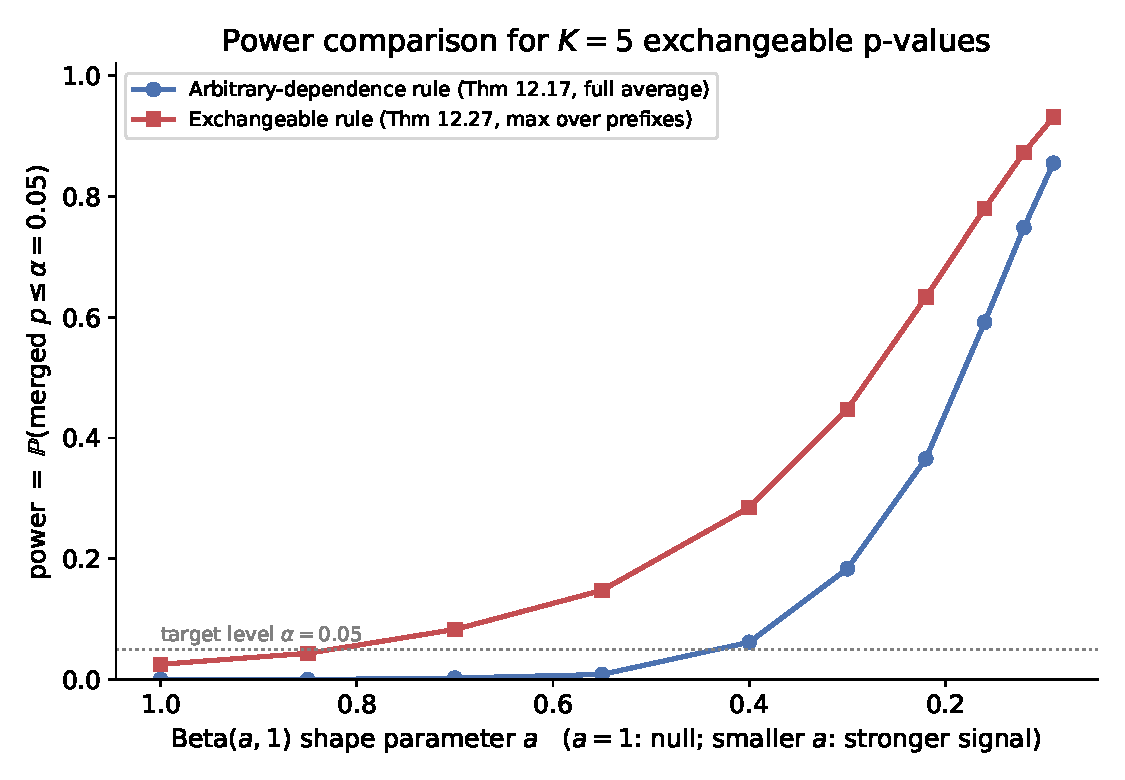
\includegraphics[width=0.82\linewidth]{fig_exchangeable_power.pdf}\\
  \small $K=5$ exchangeable p-values simulated as i.i.d.\ $\mathrm{Beta}(a,1)$ (randomly reordered each replicate to make exchangeability, not independence, the only thing used); $a=1$ is the null, smaller $a$ means more real signal. At every signal strength, the prefix-average rule (Theorem 12.27) rejects more often than the full-average rule (Theorem 12.17) at the same nominal level $\alpha=0.05$, while both control Type-I error at $a=1$.
\end{frame}

%% =========================================================================
\begin{frame}{Section 12.4 -- Intuition: what does randomization buy us?}
  \begin{itemize}
    \item Sections 12.1--12.3 all end in a Markov-inequality step: $\PP(\bar E\ge1/\varepsilon)\le\varepsilon\cdot\EE[\bar E]\le\varepsilon$. Plain Markov compares $\bar E$ to the \emph{fixed} threshold $1/\varepsilon$.
    \item Chapter 2's \emph{randomized} Markov inequality replaces this fixed threshold with a threshold that itself depends on an independent auxiliary random variable -- this squeezes extra power out of exactly the same e-values, at the cost of injecting outside randomness that two analysts of the same data might resolve differently.
    \item This is the same idea already glimpsed in Theorem 12.8 ($\indic{P\le2\alpha U}$ is a sharper, randomized version of $\indic{2\bar P\le\alpha}$); Theorem 12.28 extends it to the fully general merging-function setting of Section 12.2.
  \end{itemize}
\end{frame}

%% =========================================================================
\begin{frame}[allowframebreaks]{12.4 Randomized combinations of p-values}
  \begin{block}{Theorem 12.28: randomized combination}
    For weights $(\lambda_1,\dots,\lambda_K)\in\Delta_K$ and calibrators $f_1,\dots,f_K$, define
    \[
      F(\bp,u) \;=\; \inf\left\{\varepsilon\in(0,1]\ :\ \sum_{k=1}^K\lambda_kf_k\Big(\frac{p_k}\varepsilon\Big)\ge u\right\}.
    \]
    Then for any p-variables $\bp$ and any p-variable $V$ \emph{independent} of $\bp$, $F(\bp,V)$ is itself a valid p-value. Validity for $U\sim\mathrm{Unif}[0,1]$ follows from the randomized Markov inequality (Ch.\ 2) applied to the e-variable $\sum_k\lambda_kf_k(P_k/\varepsilon)/\varepsilon$ in place of plain Markov's inequality; validity for a general independent p-variable $V$ then follows since $F(\bp,u)$ is increasing in $u$, so $\PP(F(\bp,V)\le\alpha)\le\PP(F(\bp,U)\le\alpha)\le\alpha$.
  \end{block}

  \begin{block}{Practical remedy when randomization is undesirable}
    If one of the inputs, say $P_k$, is known to be independent of the rest, you can set $V=P_k$ itself (no extra coin flip needed) and merge the remaining $K-1$ p-values with randomization ``for free.'' Otherwise, if randomization is permitted at all, apply the exchangeable rule of Section 12.3 to a \emph{randomly permuted} ordering of the arbitrarily-dependent p-values -- turning Section 12.2's problem into Section 12.3's easier one.
  \end{block}

  \framebreak

  \begin{block}{Table 12.29 -- summary of all combination rules in this chapter}
    \begin{center}
    \small
    \begin{tabular}{@{}lccc@{}}
      \toprule
       & Arbitrary dep.\ (12.2) & Exchangeable (12.3) & Arbitrary, randomized (12.4) \\
      \midrule
      Order stats & $\tfrac Kk p_{(k)}$ & $\tfrac Kk\bigwedge_{m}p^m_{(\lambda_m)}$ & $\tfrac Kk p_{(\lceil Uk\rceil)}$ \\
      Arithmetic mean & $2\,\mathbb{M}_1(\bp)$ & $2\bigwedge_m\mathbb{M}_1(\bp_m)$ & $\tfrac2{2-U}\mathbb{M}_1(\bp)$ \\
      Geometric mean & $\mathrm{e}\,\mathbb{M}_0(\bp)$ & $\mathrm{e}\bigwedge_m\mathbb{M}_0(\bp_m)$ & $\mathrm{e}^U\mathbb{M}_0(\bp)$ \\
      Harmonic mean & $(T_K{+}1)\mathbb{M}_{-1}(\bp)$ & $(T_K{+}1)\bigwedge_m\mathbb{M}_{-1}(\bp_m)$ & $(T_KU{+}1)\mathbb{M}_{-1}(\bp)$ \\
      \bottomrule
    \end{tabular}
    \end{center}
    Here $U\sim\mathrm{Unif}[0,1]$ independent, $T_K=\log K+\log\log K+1$, and $\bp_m$ denotes the first $m$ p-values -- randomization (rightmost column) improves the arbitrary-dependence rules using the very same machinery as the exchangeable rules, but without needing an exchangeability assumption.
  \end{block}
\end{frame}

%% =========================================================================
\begin{frame}{Running example, part 4: what randomization buys, in numbers}
  \begin{block}{Same $K=4$ numbers, now allowing an independent draw $U\sim\mathrm{Unif}[0,1]$}
    Using the randomized version of Theorem 12.28 with $f(p)=(2-2p)_+$, solve $\tfrac14\sum_kf(p_k/\varepsilon)\ge u$ for the drawn value of $u$:
    \[
      \begin{array}{ll}
        u=1.0\ (\text{no randomization, back to Thm 12.17}): & F(\bp,1)=0.47,\\[2pt]
        u=0.5: & F(\bp,0.5)=0.17,\\[2pt]
        u=0.3: & F(\bp,0.3)=0.05,\\[2pt]
        u=0.1: & F(\bp,0.1)=0.025.
      \end{array}
    \]
  \end{block}
  \begin{block}{Interpretation}
    A \emph{smaller} realized draw $u$ (which happens with probability $u$ under $U\sim\mathrm{Unif}[0,1]$) gives a \emph{smaller}, more powerful merged p-value -- but validity is only guaranteed on \emph{average over the randomness of $U$}: the randomized Markov inequality ensures $\PP(F(\bp,U)\le\alpha)\le\alpha$ still holds after integrating out $U$, even though any single realized $u$ can look either lucky or unlucky.
  \end{block}
\end{frame}

%% =========================================================================
\begin{frame}{Chapter 12 summary}
  \begin{itemize}
    \item \textbf{12.1}: the arithmetic mean of p-values is not itself a p-value, but \emph{twice} the mean always is (Prop.\ 12.4) -- and this ``$2$'' is exactly the constant forced by a convex p-to-e calibrator $f(p)=(2-2p)_+$ combined with Markov's inequality (Thm.\ 12.6). Average p-values sit strictly between p-values and e-values in the calibration hierarchy.
    \item \textbf{12.2}: \emph{every} admissible way of merging p-values under arbitrary dependence secretly factors through merging e-values via calibrators and weights, then applying Markov's inequality (Thm.\ 12.15, 12.17) -- this is not one trick among many, it is the \emph{only} trick.
    \item \textbf{12.3}: exchangeability alone does not help \emph{symmetric} rules (Prop.\ 12.26) -- but deliberately breaking symmetry via running/prefix averages (Thm.\ 12.27), justified precisely because exchangeable data doesn't care about order, gives a strict, free improvement.
    \item \textbf{12.4}: randomization upgrades Markov's inequality to a randomized version (Thm.\ 12.28), buying further power from arbitrarily dependent p-values without any distributional assumption, at the cost of extra external randomness.
    \item \textbf{Running numeral:} $p=(0.02,0.15,0.30,0.60)$ merges to $0.535$ (classical $2\times$mean), $0.47$ (admissible arbitrary-dependence rule), $0.04$ (exploiting exchangeability), or as low as $0.025$--$0.05$ (with randomization) -- the \emph{same} four numbers, four increasingly sharp but always-valid answers, depending on what you are willing to assume or randomize.
  \end{itemize}
\end{frame}

\end{document}
